\documentclass{hwz}
% custom colors
\definecolor{ccc}{rgb}{0.8,0.8,0.8}

% AXA (insipred) colors
\definecolor{igloo}{rgb}{0.7,0.81,0.93}
\definecolor{igloo-darker}{rgb}{0.2,0.3,0.43}
% \usepackage{showframe}

% charts 
\usepackage{pgfplots}
\usetikzlibrary{external}
\tikzexternalize[prefix=tikz/]

% floating figures/tables
\usepackage{wrapfig}

% charts (e.g. flowcharts)
\usepackage{tikz}
\usetikzlibrary{positioning} % for right=of ... syntax
\usetikzlibrary{shapes.geometric, arrows}
\tikzstyle{startstop} = [rectangle, rounded corners, minimum width=3cm, minimum height=1cm,text centered, draw=black, fill=red!30]
\tikzstyle{io} = [trapezium, trapezium left angle=70, trapezium right angle=110, minimum width=3cm, minimum height=1cm, text centered, draw=black, fill=blue!30]
\tikzstyle{process} = [rectangle, minimum width=3cm, minimum height=1cm, text centered, draw=igloo-darker, fill=igloo!50]
\tikzstyle{process2} = [rectangle, minimum width=3cm, minimum height=1cm, text centered, draw=igloo-darker, fill=igloo!100]
\tikzstyle{decision} = [diamond, minimum width=3cm, minimum height=1cm, text centered, draw=black, fill=green!30]
\tikzstyle{arrow} = [thick,->,>=stealth]

\begin{document}

%#############################
% Title page
%#############################
\begin{titlepage}
    {
    	\centering
    	
    	\vspace*{2cm}
    	% \includegraphics[width=0.15\textwidth]{example-image-1x1}\par\vspace{1cm}
    	{\Large\fontfamily{ppl}\selectfont Grobkonzept zur Bachelor Thesis}
    	
    	{\LARGE\bfseries\fontfamily{ppl}\selectfont Automatisierung von Geschäftsprozessen durch künstliche Intelligenz am Beispiel der Rechnungsindexierung in der Krankenversicherung \par}
    	
    	\vspace{3cm}
    	
    	{Zürcher Fachhochschule\par}
    	
    	{\bfseries\large\fontfamily{ppl}\selectfont HWZ Hochschule für Wirtschaft Zürich\par}
    	
    	\vfill
    }
    {
        \renewcommand{\arraystretch}{1.5}
        \setlength{\tabcolsep}{0pt}
        \begin{flushleft}
    	\begin{tabular}{ l@{\hspace{1.5cm}} l }
         Student: & Sven Tschui \\
         Studiengruppe: & BWI-A15 \\
         Betreuungsperson: & Dr. Oliver Zenklusen \\
         Datum & 1. Dezember 2018 \\
        \end{tabular}
        \end{flushleft}
    }
\end{titlepage}

\newpage

%#############################
% TOC
%#############################
\tableofcontents

\newpage

\makeBeginMain

%#############################
% Ausgangslage
%#############################
\section{Ausgangslage, Forschungsproblem und -frage}

\todo[inline]{
In der Ausgangslage wird das Thema zuerst allgemein vorgestellt, dann wird auf einen bestimmten Teilaspekt des Themengebiets fokussiert. 

Diese Fokussierung führt zum Forschungsproblem und damit zu den Erkenntnissen, die gewonnen werden sollen. Gründe werden aufgeführt, weshalb es relevant ist, das gewählte Problem zu untersuchen. Ausserdem wird der Wissensstand im Bereich des Forschungsproblems (was weiss man bereits, was noch nicht) knapp beschrieben. 

Die Forschungsfrage schliesslich bündelt die zentralen Aspekte des Forschungsproblems als zugespitzte Frage. Die Frage sollte bereits so konkret sein, dass sie in einer Thesis untersucht werden kann.

\textit{(Bitte diesen Text jeweils nicht löschen. Er dient als Information für die Betreuungsperson.)}
}

% Schneller und guter Kundenservice ist wichtig um Kunden halten zu können, dies ist längst bekannt \todo{CITE}. Auch die Auswirkungen einer hohen Kundenzufriedenheit auf die Kundenloyalität werden als sehr stark anerkannt \todo{CITE}. Aus diesen Gründen investieren Unternehmen immer stärker in diese Services und versuchen sich damit von der Konkurrenz zu differenzieren \todo{CITE}. Diese Services bereitzustellen kann für ein Unternehmen sehr kostenintensiv sein \todo{CITE}. \todo[inline, color=orange]{ Fakten und Zahlen würden diese Aussage nicht nur untermauern sondern auch spannender machen} Kundenservices sollen heutzutage mit geeigneter Soft- und Hardware automatisiert werden, um die Kosten so gering wie möglich zu halten \todo{CITE}. Die Automatisierung hat ausserdem den Effekt, dass Services schneller abgewickelt werden können, was im Zeitalter der ungeduldigen Kunden ein wichtiger Differenzierungsfaktor sein kann \todo{CITE}. Die Automatisierung durch klassische Software stösst aber teilweise \todo{konkrekt sagen, wann diese Grenzen auftreten} an ihre Grenzen. Die klassische, strukturierte Programmierweise bildet Logik ab, welche durch Ursache-Wirkung klar definierbar ist: Wenn eine Bedingung eintrifft, wird etwas ausgeführt \todo{QUOTE}. Ein Abwägen von Fall zu Fall, wie dies ein Angestellter im Kundenservice machen könnte, ist mit solcher Software nicht möglich. Eine Lösung für diese Limitierung bietet die künstliche Intelligenz: Der Computer wird nicht mehr angewiesen was zu tun ist, sondern was das Ziel ist. Der Computer wird dann auf die erreichung dieses Ziels trainiert \todo{QUOTE}.

% In dieser Arbeit werden die Möglichkeiten diskutiert, welche die künstliche Intelligenz für die Automatisierung von Kundenservices bietet. Im ersten Teil werden die grundlegenden Elemente der Künstlichen Intelligenz erläutert und Herausforderungen in der Automatisierung der Kundenservices aufgezeigt. \todo[inline]{weiterer Inhalt, e.g. theoretische erfahrung, Praxisbeispiele} Der zweite Teil widmet sich einem Fallbeispiel eines Kundenservices, welcher in einem Prototypen durch den Einsatz von Künstlicher Intelligenz automatisiert werden soll. Der Erfolg des Experiments wird anhand zuvor definierten Erfolgskriterien diskutiert.

% \subsection{Fallbeispiel}

Die Anwendung der künstlichen Intelligenz zur Automatisierung von Aufgaben wird in einigen Branchen bereits diskutiert. Im Bereich der Landwirtschaft gibt es bereits mehrere Studien, welche die Lösung der Problematiken der Krankheitserkennung, Saatgutqualität sowie der Phänotypisierung unter Anwendung von computergestützter Bildverarbeitung mit künstlicher Intelligenz in der Produktion von Saatgut, diskutieren~\autocite{Patricio2018ComputerReview}. 

Um die Produktion des neuen Airbus A350 schnellstmöglich auf Hochtouren zu bringen wurde künstliche Intelligenz angewendet. Ein System, welches von Airbus entwickelt wurde, ermöglicht dank künstlicher Intelligenz, in 70\% aller Unterbrüche der Produktion in kürzester Zeit eine Lösung auszuarbeiten~\autocite{Ransbotham2017ReshapingIntelligence}.

Auch Ping An Insurance Co. of China Ltd., eine der grössten Versicherungsgesellschaften von China, verwendet bereits künstliche Intelligenz zur Automatisierung von diversen Kundenservices~\autocite{Ransbotham2017ReshapingIntelligence}.

Neben diesen Pionieren erwähnen \textcite{Ransbotham2017ReshapingIntelligence} in Ihrer Untersuchung aber auch, dass nur 14\% der Befragten denken, dass künstliche Intelligenz aktuell einen hohen Einfluss auf Ihre Angebote und Dienstleistungen haben. Jedoch denken 63\%, dass sich dies in den nächsten 5 Jahren ändern wird und die künstliche Intelligenz ein entscheidender Wettbewerbsvorteil bieten kann. Trotz des Verständnis der künstlichen Intelligenz und des Potential einen Wettbewerbsvorteil zu schaffen, wird diese noch zu wenig angewendet\autocite{Ransbotham2017ReshapingIntelligence}.

Auch im \textcite{TheEconomist2018TheAI} wird der mögliche Wettbewerbsvorteil durch die Anwendung von künstlicher Intelligenz angesprochen. Auch ausserhalb des Technologie-Sketors, in Branchen, welche aktuell durch den Konkurrenzkampf geprägt sind, werden grosse Firmen durch die anwendung künstliche Intelligenz noch grösser und entwickeln sich zu Monopolen~\autocite{TheEconomist2018TheAI}.

\subsection{Potential der künstlichen Intelligenz bei der AXA Gesundheitsvorsorge}

In diesem Kapitel wird ein Fallbeispiel beschrieben, in welchem die Anwendung künstlicher Intelligenz einen Wettbewerbsvorteil haben könnte. Dieser Fall wird für den Arbeitgeber des Autor, die AXA Gesundheitsvorsorge, untersucht. Einige der Aussagen in diesem Kapitel werden basieren auf der Berufserfahrung des Autoren getroffen.

In der Schweiz beliefen sich die Kosten für das Gesundheitswesen im Jahr 2015 auf 77.8 Milliarden Franken. Über 35\% dieser Kosten wurden durch die obligatorische Krankenversicherung gedeckt. Weitere knapp 7\% wurden von den Zusatzversicherungen übernommen. Die Krankenversicherer finanzierten also mit knapp 42\% einen beträchtlichen Teil des Gesundheitswesens in der Schweiz \autocite{BfS2018Finanzierung, BfS2017KostenDaten}.

Die Kosten des Gesundheitswesen steigen stetig an, so weisen die Zahlen vom Jahr 2016 bereits Kosten von über 80 Milliarden Franken nach. Auch in den folgenden Jahren sollen die Kosten weiter steigen. \textcite{Kirchgassner2009DasKostenentwicklung} begründet diesen Anstieg unter anderem mit der Veränderung der Altersstruktur, dem steigenden Wohlstand sowie den neuen Möglichkeiten in der Diagnose und Behandlung durch technischen Fortschritt~\autocite{BfS2018Finanzierung, Kirchgassner2009DasKostenentwicklung}.

Die Kosten, welche die Krankenversicherer tragen, werden mit einem von zwei Systemen, \textit{Tiers payant} oder \textit{Tiers garant}, vergütet \autocite{EDI2017FaktenblattVergutungssysteme}. 

\begin{wraptable}{l}{0.53\textwidth}
    \renewcommand{\arraystretch}{1.25}
    \setlength{\tabcolsep}{5pt}
    \caption{Vergütungsmodelle bei den schweizer Krankenversicherern}
    \begin{tabular}{| p{0.15\textwidth} | p{0.32\textwidth} |}
        \hline
         Tier payant & Kosten werden vom Leistungserbringer direkt dem Krankenversicherer in Rechnung gestellt. \\
        \hline
         Tier garant & Kosten werden vom Leistungserbringer dem Patienten in Rechnunge gestellt, welcher die Rechnung dem Krankenversicherer zur Rückvergütung weiterleitet. \\
        \hline
    \end{tabular}
\end{wraptable}

Beim System Tier payant belastet der Leistungserbringer (bspw. Arzt oder Apotheke) die Kosten direkt dem Krankenversicherer. Dies geschieht, in dem der Patient mit seiner Versichertenkarte bezahlt. Anhand dieser Versichertenkarte, welche vom Krankenversicherer ausgestellt wird, können Deckungen für den Patienten überprüft sowie die Rechnung direkt an den Krankenversicherer übermittelt werden. In diesem Fall wird die Rechnung bereits in digitaler, strukturierter Form übermittelt und der Krankenversicherer kann mit einem entsprechenden Regelwerk die Rechnung automatisch verarbeiten~\autocite{EDI2017FaktenblattVergutungssysteme, BAG2016AntwortenVersichertenkarte}. 

Werden Kosten, welche über Tier payant abgerechnet wurden, nicht vom Krankenversicherer getragen, weil beispielsweise ein Selbstbehalt vereinbart wurde, die Franchise noch nicht aufgebraucht ist oder der Patient für diese Behandlung gar nicht versichert ist, verrechnet der Krankenversicherer die Kosten dem Patienten weiter \autocite{EDI2017FaktenblattVergutungssysteme}.

Das System Tier payant wird häufig in Apotheken, beim Kauf von Medikamenten mit oder ohne ärztlichem Rezept, sowie bei allen stationären Behandlungen, gemäss Art. 42 Abs. 2 KVG, verwendet \autocite{EDI2017FaktenblattVergutungssysteme}.

Die Verarbeitung von Rechnungen, welche über das System Tier payant abgerechnet werden, kann der Krankenversicherer, aufgrund der digitalen, strukturierten Daten, automatisiert gestalten~\autocite{BAG2016AntwortenVersichertenkarte}.

Im Fall von Tiers garant stellt der Leistungserbringer die Rechnung direkt dem Patienten aus, welcher diese dann seinem Krankenversicherer zur Rückerstattung weiterleitet. Die Rechnung kann bei allen Krankenversicherern per Post und bei den meisten auch digital, im Kundenportal oder in der App, eingereicht werden \autocite{EDI2017FaktenblattVergutungssysteme}.

Rechnungen, welche per Post oder digital beim Krankenversicherer zur Rückvergütung eingehen, erreichen diesen in verschiedenen Formen und unterschiedlichster Qualität. 

Während einige Rechnungen nach dem TARMED Standard für Rückforderungsbelege strukturiert sind, sind andere formlos. Die Bandbreite an Formen ist hier gross: Von handgeschriebenen Rechnungen eines örtlichen Leistungserbringer bis hin zu strukturierten Rechnungen von Fitnessketten.

Bei der Einreichung per Post kann die Qualität durch Kaffee-Flecken, Verbleichung der Belege oder sonstige Beeinträchtigungen gemindert werden, der Krankenversicherer kann aber einiges dazu beitragen die Rechnung in hoher Qualität einzulesen. So kann er beispielsweise hochauflösende Scanner und eine optimale Beleuchtung einsetzen.

Problematischer sind Rechnungen, welche von Kund/-innen digital, sprich als Photo, an den Krankenversicherer übermittelt werden. Wird ein Foto einer Rechnung über das Kundenportal eingereicht, so hat der Krankenversicherer nur noch sehr wenig Einfluss auf die Qualität der Aufnahme. Schlechte Belichtung, kleine Auflösung und abgeschnittene Rechnungen sind nur wenige der Probleme, mit welchen der Krankenversicherer zu kämpfen hat.

Egal wie und in welcher Qualität eine Rechnung einen Krankenversicherer erreicht hat, muss dieser die Rechnung in eine elektronische, strukturierte Form bringen, damit diese dann durch ein Regelwerk verarbeitet werden kann. Dieser Vorgang wird durch verschiedenste Techniken aus den Bereich der Texterkennung und der Informationsextraktion ermöglicht. Als Texterkennung oder auch Optical Character Recongition (kurz OCR) wird ein Vorgang bezeichnet, bei welchem Handschrift oder Druckbuchstaben in eine Form gebracht werden, welche von Maschinen verstanden und bearbeitet werden kann~\autocite{Xue2014OpticalRecognition}. Unter dem Begriff Informationsextraktion oder Information extraction (kurz IE) wird der Prozess verstanden, bei welchem relevante Fakten aus einem Text gewonnen werden~\autocite{Piskorski2012InformationFuture}.

% \todo[inline, color=green]{Wie macht das die Post? Postfinance? Dort ist das Problem vermutlich etwas einfacher aber Lösungen gibt es schon länger?}

% Viele Krankenkassen haben diese Technologien bereits im Einsatz. Auch gibt es diverse Anbieter, wie beispielsweise die Tessi document solutions (Switzerland) GmbH oder die Cent Systems AG, welche diese Technologien oder gar umfangreiche Services in diesem Bereich anbieten. Die Erfahrung mit diesen Technologien und Providern bei der AXA Ein grosser Teil der Rechnungen muss aber, aus verschiedenen Gründen, nach wie vor manuell bearbeitet werden \todo{Quelle für manuelle arbeiten}. Dies beinhaltet sowohl die Nachbearbeitung nach der elektronischen Indexierung als auch die komplett manuelle Indexierung\todo{CITE}. 
% Die CSS Krankenkasse beschäftigt beispielsweise rund 200 Personen für diese manuelle Indexierung. Bei der Assura sind es rund 500 Personen \todo{Quelle für die Anzahl personen}.

% Im Jahr 2016 wiesen die Grundversicherer einen durchschnittlichen Verwaltungskostensatz von 4.7\% aus. Dies bedeutet  Ein guter Verwaltungskostensatz konnte die CSS Kranken-Versicherung AG im Jahr 2017 ausweisen weist im Jahr Die Indexierung dieser Rechnungen ist einer der Faktoren, welche auf die hohen Verwaltungskosten der Krankenversicherer schlägt.

Die AXA, eine internationale Versicherungsgesellschaft, sieht sich, genau wie alle anderen Krankenversicherer, ebenfalls vor der Herausforderung der Indexierung von Rechnungen. Im Jahr 2017 lancierte die AXA eine Zusatzversicherung in der Gesundheitsvorsorge im Schweizer Markt. Neben der Zusatzversicherungen selbst bietet die AXA ihren Kunden einen Rechnungs-Weiterleitungs-Service. Das bedeutet, alle Rechnungen können der AXA gesendet werden. Rechnungen beziehungsweise Rechnungspositionen, welche die Zusatzversicherung betreffen, werden von der AXA vergütet und Rechnungspositionen, welche die Grundversicherung betreffen, werden zur Vergütung an den Grundversicherer weitergeleitet \autocite{finanzen.ch2017AxaGewinnen}.

Gemäss einem Beitrag auf \textcite{finanzen.ch2017AxaGewinnen} ist es das Ziel der AXA, bis im Jahr 2020 insgesamt 100'000 Kunden für die Gesundheitsvorsorge zu gewinnen. Aus dem Geschäftsbericht der CSS Gruppe für das Jahr 2017 geht hervor, dass für knapp 1.7 Millionen Kunden 16 Millionen Rechnungen geprüft wurden~ \autocite{CSSGruppe2018Geschaftsbericht2017}. Werden die durchschnittlich 9.5 Rechnungen pro Kunde auf die Zielgrösse 100'000 Kunden der AXA hochgerechnet, so muss die AXA im Jahr 2020 knapp 1 Million Rechnungen prüfen. Damit diese Menge an Rechnungen effizient verarbeitet werden kann, ist es für die AXA wichtig, den Prozess der Indexierung möglichst automatisiert zu gestalten.

Um die Verwaltungskosten der Zusatzversicherung aufzuzeigen wird wiederum der Ge\-schäfts\-be\-richt der CSS Gruppe für das Jahr 2017 herangezogen. Der Kostensatz, welcher der Anteil der Gemeinkosten am Umsatz misst, für die Grundversicherung betrug lediglich 4\%. Im Geschäftsbereich der Zusatzverischerung liegt dieser Kostensatz allerdings viel höher, nämlich bei 21\%. Welcher Anteil an diesen Kosten nun der Prüfung respektive der Indexierung eingehender Rechnungen zuzuschreiben ist, bleibt ein Betriebsgeheimnis. Da die Rechnungen, welche die Zusatzversicherungen betreffen, aufgrund der unterschiedlichen Leistungserbringer (Alternativmedizin, Fitness, Sportvrein) viel diverser sind als jene die die Grundversicherung (Ärzte und Spitäler nach TARMED standard) betreffen, liegt die Vermutung nahe, dass im Bereich der Zusatzversicherung ein hoher Anteil der Verwaltungskosten der Rechnungsprüfung zugeschrieben werden kann.

Die AXA profitiert aber bei einer automatisierten Indexierung von Rechnungen nicht nur von einer Kostensenkung sondern kann damit auch einen Vorteil für Ihre Kunden generieren: Die Kunden erhalten durch die automatisierte Verarbeitung der eingereichten Rechnungen viel schneller das geforderte Geld.

%Rechnungen, egal ob diese von der AXA selbst bezahlt oder an den Grundversicherer weitergeleitet werden, müssen indexiert werden um verarbeitet werden zu können. Die Indexierung wird aktuell von einem externen Provider übernommen und ist eine \todo[color=yellow]{erläutern}Blackbox. Es ist allerdings bekannt, dass ein grosser Teil der Arbeiten, nach einem automatisierten OCR Schritt, manuell gemacht werden. Die aktuelle Indexierung birgt folgende zwei Probleme:

%\todo[inline, color=igloo]{Hinweis: Ich weiss, ist eine provokative Frage. Aber ich frage mich, ob es Sinn macht, dies so zu erwähnen, weil daraus entstehen Fragen -> Warum dieser Provider, wenn nicht klar ist, was er macht? Oder warum wird nicht das Know-how akquiriert?}

%\todo[inline, color=igloo]{Frage: Warum müssen die Rechnungen indexiert werden? Bitte kurz erklären, warum dies Unternehmen machen. }

Aus der aktuell halb-automatisierten Indexierung von Rechnungen bei der AXA kann gesagt werden, dass für die Automatisierung auf folgende zwei Punkte geachtet werden muss:

\begin{itemize}
    \item Qualität der Indexierten Daten: Fehler in der Indexierung (z.B. 1g anstelle 500mg Tabletten) führen zu Fehlern in den Abrechnungen, welche im schlimmsten Fall eine Benachteiligung des Kunden verursachen und somit das Vertrauen des Kunden beeinträchtigen.
    \item Manueller Aufwand: Ein hoher Anteil an manueller Arbeit verursacht hohe Kosten, ist nicht effizient, birgt viel Potential für Fehler und kann nicht schnell skaliert werden.
\end{itemize}

% \todo[inline, color=green]{Problematik von Anfang an prägnanter darstellen? (Der aufwändige Schritt „Indexierung“ im erwähnten Prozess? Was ist das Problem? Warum braucht es Ihr Projekt?)}

In dieser Arbeit wird diskutiert, ob die Indexierung der eingehenden Rechnungen durch die Anwendung von künstlicher Intelligenz automatisiert werden kann.

Für die Problemstellung ist es nicht nur relevant ob sondern auch in welcher Qualität dieser Arbeitsschritt automatisiert werden kann. Die Qualität stellt ein wichtiger Punkt dar, da schlechte Qualität ein Image-Schaden und somit ein Wettbewerbsnachteil nach sich ziehen könnte.

Aufgrund der geschilderten Problematik der Indexierung von Rechnungen bei der AXA entstand die Idee, diese mit neuen Technologien zu lösen. Aus dem beschriebenen Fallbeispiel und dem branchenübergreifenden Interesse an der Anwendung der künstliche Intelligenz zur Automatisierung von Geschäftsprozessen wird für diese Arbeit folgende Forschungsfrage definiert.

{
    \medskip
    \setlength{\fboxsep}{1em}
    \noindent\fcolorbox{igloo-darker}{igloo}{%
        \minipage[t]{\linewidth-2\fboxsep-2\fboxrule\relax}
            \begin{flushleft}
                \centering
                Können Geschäftsprozesse durch Künstliche Intelligenz automatisiert werden?
            \end{flushleft}
        \endminipage}
    \medskip
}

Um die Beantwortung dieser Forschungsfrage zu untersützen, werden folgende Unterfragen abgeleitet:

\begin{itemize}
    \item Was wird unter künstlicher Intelligenz verstanden?
    \item Was ist die Rechnnungsindexierung und welche Rolle spielt diese für einen Krankenversicherer?
    \item Welche Ansätze aus dem Bereich der künstlichen Intelligenz können für die Rechnungsindexierung angewendet werden?
\end{itemize}

%
%
%
%
%
% TODO: Diskussion für KI vs ML
%
%
%
%
%
%

\subsection{Forschungsstand}

% \todo[inline, color=igloo]{Vorschlag: Hier könntest Du mit dem Begriff "KI" beginnen und die Problematik ansprechen, dass zwar viele davon sprechen, aber (falls überhaupt) nur wenige wissen, was darunter zu verstehen ist. Vieles, was heute angeboten wird, basiert auf ML-Ansätzen, wie z.B. und dann kannst Du best practices aufweisen.}

Die künstliche Intelligenz ist ein sehr aktuelles und deshalb auch in der Literatur oft diskutiertes Themengebiet. Bereits 2009 geben \textcite{Russell2009ArtificialEdition} auf über 1000 Seiten einen noch immer aktuellen und sehr umfangreichen Überblick über das Themengebiet. Weiter vertiefen die beiden Autoren viele Teilgebiete der künstlichen Intelligenz und erläutern Grundlegende Konzepte ausführlich.

Einen etwas mathematischeren Überblick über das Thema künstliche Intelligenz geben \textcite{Goodfellow2016DeepLearning}. Die Dikussion reicht von den absoluten Grundlagen, der linearen Algebra, bis hin zu Deep Generative Models, eine fortgeschrittene Anwendung der künstlichen Intelligenz~\autocite{Goodfellow2016DeepLearning}.

Zusammenfassend kann gesagt werden, dass in der Grundlagenforschung zur künstlichen Intelligenz bereits viele Forschungsergebnisse vorliegen. Es werden etliche, etablierte und experimentelle, Techniken diskutiert. Für die Entwicklung des Prototypen für die AXA stehen somit viele Möglichkeiten zur Verfügung.

Um einen ersten Überblick über die Problemstellung zu erhalten, werden einige Techniken im Bereich der künstlichen Intelligenz, welche für die Beantwortung der Forschungsfrage sowie für die Entwicklung des Prototypen relevant sind, in den folgenden Kapiteln erkundet.

\subsubsection{Neuronale Netzwerke}

Abgesehen von Rechenaufgaben sind Menschen Leistungsfähiger als Computer. Wir sind beispielsweise in der Lage, Gesichter zu erkennen oder in einem dunklen Raum Personen anhand Ihrer Stimme zu identifizieren. Der interessanteste Unterschied des Menschlichen Gehirns zu einem Computer ist allerdings der Fakt, dass unser Gehirn lernt ohne ein Software-Update zu erhalten. Wir brauchen nicht erst eine neue Software um das Fahrradfahren zu erlernen. Doch wie funktioniert das~\autocite{Krogh2008WhatNetworks}?

Die Berechnungen unseres Gehirn werden durch hoch vernetzte Neuronen gemacht. Dabei interagieren die Neuronen mit Stromimpulsen durch die Neuronale Verkabelung, bestehend aus Nervensäulen, Synapsen und Zellfortsätzen. 1943 Modellierten McCulloch und Pitts Neuronen als Schalter, welche aufgrund der eingehenden Signale Ein- oder Ausgeschaltet sind. Die Gewichtung der eingehenden Signale waren dabei die Synapsen. Neuronale Netzwerke sind also inspiriert von den ersten Modellen des menschlichen Gehirns~\autocite{Krogh2008WhatNetworks}.

Damit ein Neuronales Netzwerk Leistungsfähig werden kann, muss es ähnlich wie ein Mensch, aber erst lernen. Das computersimulierte Lernen, auch Machine Learning genannt, funktioniert dabei so, dass für die Gewichte der Verbindungen, sprich die stärke der Synpasen, ein zufälliger Wert gewählt wird. Anschliessend wird eine Beispielaufgabe vom Netzwerk gelöst. Das Resultate des Netzwerks ist zu Beginn höchstwahrscheinlich falsch und die Gewichte im Netzwerk werden mit einem kleinen Schritt angepasst. Es werden dann immer weitere Beispielaufgaben gelöst und die Gewichte entsprechend angepasst bis das Netzwerk die gewünschten Resultate liefert~\autocite{Krogh2008WhatNetworks}.

Seit mehreren Jahren liefern Neuronale Netzwerke bessere Resultate als andere Techniken. Dabei werden Neuronale Netzwerk vorwiegend für visuelle Tasks und immer häufiger auch zur Verarbeitung Natürlicher Sprache verwendet~\autocite{Olah2014DeepRepresentations}.

\todo[inline]{Say a word on overfitting}

\todo[inline]{Say something about learning strategies (supervised / unsupervised)}

\subsubsection{LSTM Netzwerke}

\todo[inline,color=red]{Bla bla...}

\subsubsection{Texterkennung}

Ein wichtiger Bestandteil des Prototypen zur Indexierung von Rechnungen ist die Erkennung von Texten, ob Druckbuchstaben oder Handschrift, auf den Rechnungen. Die erkannten Texte bilden die Grundlage für jegliche digitale Verarbeitung der Rechnungen.

Die feature-detection in Texterkennungssoftware wird immer mehr mit künstlicher Intelligenz ersetzt. \textcite{Neuberg2017CreatingLearning} beschreibt wie Dropbox künstliche Intelligenz anwendet, um Texte aus Photographien von Dokumenten durchsuchbar zu machen. Zur Anwendung kommen dabei verschiedene Techniken aus dem Bereich der künstlichen Intelligenz: \textit{Convolutional Neural Network} (CNNs),  \textit{Long-Short-Term-Memory} (LSTM) Netzwerke, \textit{Connectionist Temporal Classification} (CTC) und mehr~\autocite{Neuberg2017CreatingLearning}.

\todo[inline, color=red]{Beschreibung von LSTM, CTC und CNN

Inline etwas ungünstig für den lesefluss... "Tabelle" sinnvoll?}

Auch die Texterkennungssoftware Tesseract, welche ursprünglich als PhD Forschungsprojekt im HP Lab entwickelt wurde und seit 2005 als Open Source Software zur freien verfügung steht verwendet seit Version 4 künstliche Intelligenz~\autocite{Smith2007AnEngine, o.V.20184.0LSTM}. So wurde die feature detecion durch ein LSTM Netzwerk mit mehr als 100 Schichten ersetzt. Die Texterkennung konnte so nicht nur Qualitativ stark verbessert werden sondern ist auch einiges schneller als zuvor. Doch auch nach den Verbesserungen sind die Ergebnisse nicht perfekt und müssen fallspezifisch optimiert werden~\autocite{o.V.20184.0Performance, o.V.20184.0LSTM}.

\subsubsection{Word embedding}

Neuronale Netzwerke funktionieren mit Zahlen, damit auch Wörter und ganze Sätze von solchen Netzwerken verarbeitet werden können, muss eine geeignete Repräsentation von Wörtern mit Zahlen gefunden werden. Der Prozess, mit welchem ein Wort in eine zahlen basierte Repräsentation gebracht wird, nennt sicht Word empedding~\autocite{Olah2014DeepRepresentations}.

Die ersten Word embeddings wurden von \textcite{Bengio2001Advances13} eingeführt. Trotz des schon fortgeschrittenen Alter dieses Forschungsgebiet ist es noch immer hoch interessant und in voller Fahrt~\autocite{Olah2014DeepRepresentations}.

\begin{wrapfigure}{r}{0.5\textwidth} 
    \caption{Modulares Netzwerk zur Validierung von 5-Grammen mit einer Word embedding Funktion ($W$) und einem Neuronal Netzwerk ($R$)}
    \label{wordembeddingtraining}
    \centering
    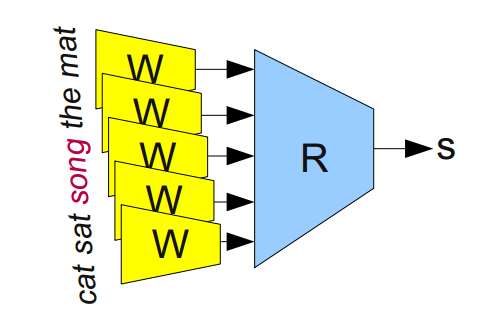
\includegraphics[width=0.48\textwidth]{graphics/wordembeddingtraining.png}
    \caption*{Quelle: \textcite{Olah2014DeepRepresentations}}
\end{wrapfigure}
Technisch gesehen ist ein Word embedding eine parametrierte Funktion, die Wörter einer bestimmten Sprache in einen hoch-dimensionalen Vektor (typischerweise 200-500 Dimensionen) transformiert. Um diese hoch komplexe Funktion zu definieren, kommt, wie bei den Neuronalen Netzwerken, Machine Learning zum Einsatz. \textcite{Olah2014NeuralTopology} beschreibt in seinem Artikel ein Beispiel, bei welchem eine solche Word embedding Funktion trainiert wird, indem die Resultate aus dem Word embedding in ein Neuronales Netzwerk zur Prüfung eines 5-Grammes (Satz mit 5 Wrötern) gespiesen werden und dann das Gesamtkonstrukt trainiert wird (vgl. Abbildung \ref{wordembeddingtraining})~\autocite{Olah2014NeuralTopology}.

Um sich Word embeddings besser vorstellen zu können, zieht \textcite{Olah2014DeepRepresentations} zwei verschiedene Visualisierungsmöglichkeiten heran~\autocite{Olah2014DeepRepresentations}.

Die erste Visualisierung bedient sich dem t-SNE Algorithmus um die hoch-dimensionalen Vektoren in einem zweidimensionalen Diagramm darzustellen. In diesem Diagramm ist klar zu erkennen, dass ähnliche Wörter nahe zusammen sind (vgl. Abbildung \ref{wordembeddingtsne}~\autocite{Olah2014DeepRepresentations}.
\begin{figure}[h]
    \centering
    \caption{t-SNE Darstellung eines Word embeddings, die verdeutlicht, dass ähnliche Wörter ähnliche Vekotren aufweisen}
    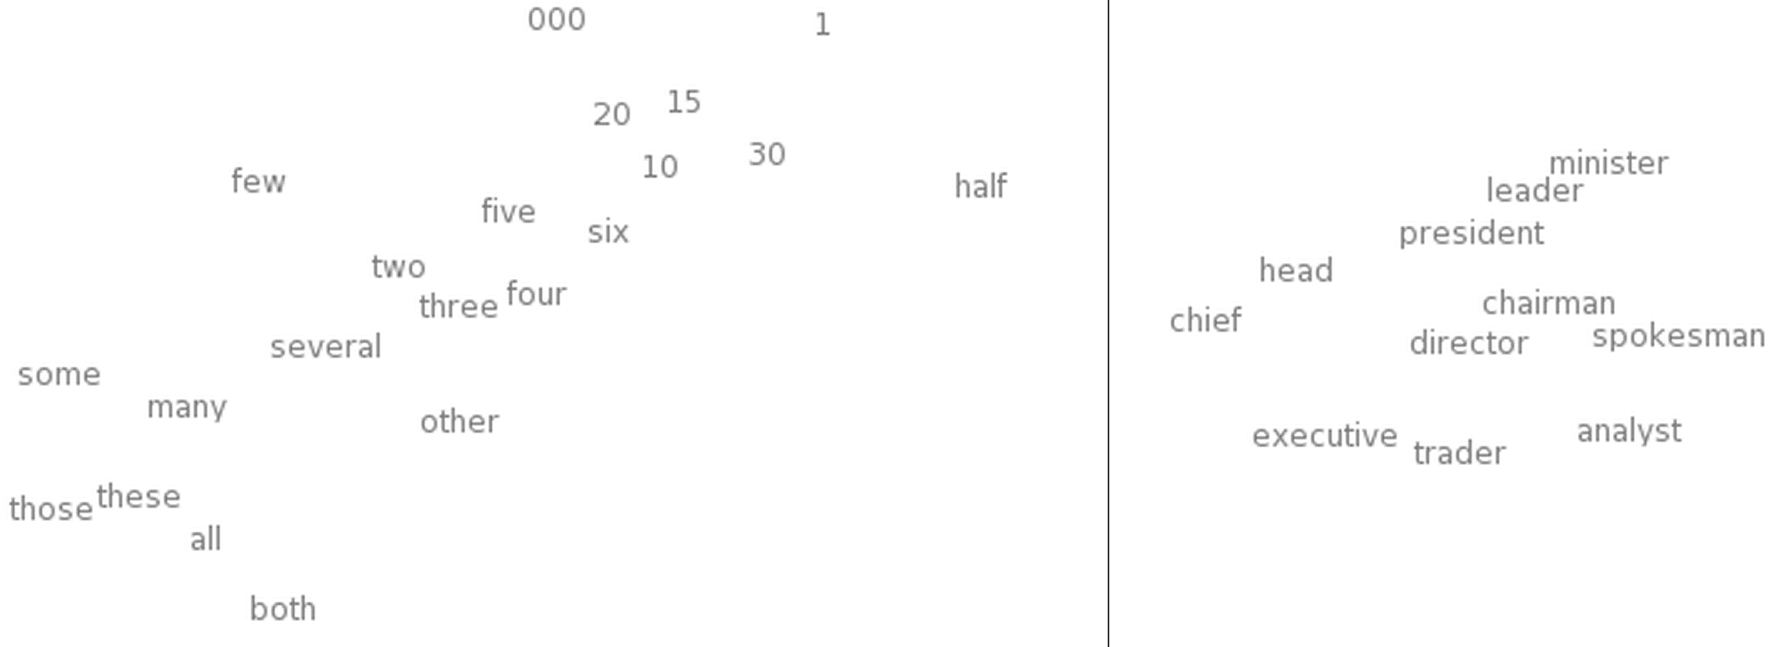
\includegraphics[width=\textwidth]{graphics/wordmebeddingtsne.png}
    \caption*{Quelle: \textcite{Turian2010WordLearning} in \textcite{Olah2014DeepRepresentations}}
    \label{wordembeddingtsne}
\end{figure}

Die zweite Visualisierung listet in einer Tabelle (vgl. Tabelle \ref{wordembeddingtable}) für sechs Wörter die nächsten Embeddings, sprich mit den mathematisch nächsten Vektoren, auf. So werden beispielsweise unter dem Titel \enquote{FRANCE} neben \textit{EUROPA} diverse weitere Länder aufgelistet.
\begin{table}[h]
\centering
    \caption{Sechs Ausgangswörter mit den ihnen ähnlichsten Word embeddings, sprich mit den mathematisch nächsten Vektoren}
    \label{wordembeddingtable}
    \renewcommand{\arraystretch}{1.25}
    \setlength{\tabcolsep}{3pt}
    \small
    \begin{tabular}{ | l | l | l | l | l | l |}
    \hline
    \rowcolor{ccc} FRANCE & JESUS & XBOX & REDDISH & SCRATCHED & MEGABITS \\ \hline
    AUSTRIA & GOD & AMIGA & GREENISH & NAILED & OCTETS \\ \hline
    BELGIUM & SATI & PLAYSTATION & BLUISH & SMASHED & MB/S \\ \hline
    GERMNAY& CHRIST & MSX & PINKISH & PUNCHED & BIT/S \\ \hline
    ITALY & SATAN & IPOD & PRUPLISH & POPPED & BAUD \\ \hline
    GREECE & KALI & SEGA & BROWNISH & CRIMPED & CARATS \\ \hline
    SWEDEN & INDRA & PS\textit{NUMBER} & GREYISH & SCRAPED & KBIT/S \\ \hline
    NORWAY & VISHNU & HD & GRAYISH & SCREWED & MEGAHERTZ \\ \hline
    EUROPE & ANANDA & DRAMCAST & WHITISH & SECTIONED & MEGAPIXELS \\ \hline
    HUNGARY & PARVATI & GEFORCE & SILVERY & SLASHED & GBIT/S \\ \hline
    SWITZERLAND & GRACE & CAPCOM & YELLOWISH & RIPPED & AMPERES \\ \hline
    \end{tabular}
    \caption*{Quelle: \textcite{Collobert2011NaturalScratch} in \textcite{Olah2014DeepRepresentations}}
\end{table}

Sowohl Abbildung \ref{wordembeddingtsne} als auch Tabelle \ref{wordembeddingtable}, zeigen die Stärke von Word embeddings auf: Ähnliche Wörter werden mit ähnlichen Vektoren versehen und somit wird eine komplexe Landschaft von Zusammengehörigen Wörtern gebildet. Aufgrund dieser Eigenschaft verändert sich durch den Austausch eines Wortes mit einem Synonym der Input Vektor für ein nachfolgendes Neuronale Netzwerk nur geringfügig, da die Word embeddings der beiden Synonyme sehr ähnlich sind. Somit muss dieses nachfolgende Neuronale Netzwerk nicht für alle Wörter der Welt trainiert werden, sondern kann auf die Generalisierung durch das Word embedding aufbauen~\autocite{Olah2014DeepRepresentations}.

Word embeddings sind zu einem extrem wichtigen Baustein bei der Verarbeitung von Natürlichen Texten geworden. Neben Input und Output Repräsentationen bei NLP Tasks können Word embeddings auch Output Repräsentationen in der Bilderkennung sein~\autocite{Olah2014DeepRepresentations}. 

Für den Prototypen bilden Word embeddings eine wichtige Grundlage, da durch diese Tehcnik die in den Rechnungen enthaltenen Wröter und Sätze in eine generalisierte, durch Neuronale Netzwerke verarbeitbare Form gebracht werden können.

\subsubsection{Korrektur von Rechtschreibung und Grammatik}

Trotz grossem Fortschritt, nicht zuletzt dank der Verwendung von künstlicher Intelligenz, im Bereich der Texterkennung, werden Texte nicht zu 100\% korrekt erkannt. So schleichen sich falsch erkannte Buchstaben ein, welche nicht nur Wörter sondern auch ganze Sätze bedeutungslos machen. Um solche Fehler zu korrigieren, wird auf die Rechtschreibung- und Grammatik-Korrektur zurückgegriffen. Während diverse Korrekturprogramme regelbasierte Software anwenden, wurde auch in diesem Bereich bereits erfolgreich künstliche Intelligenz angewandt.

Mit Hilfe der in einem vorherigen Kapiteln eingeführten Technik des Word embeddings und von LSTM Netzwerken lässt sich diese Problematik angehen. So kann ein Modulares Netzwerk aus Word embeddings und mehreren LSTM Schichten verwendet werden, um eine Rechtschreibkorrektur vorzunehmen. So beschreibt \textcite{Weiss2016DeepSpelling} in seinem Blog, wie mit einem einfachen Neuronalen Netzwerk, bestehend aus nur 4 LSTM und 4 Dropout Schichten, bereits erfolgreich Rechtschreibfehler korrigiert werden können. 

Nicht nur zur Korrektur von Rechtschreibfehler ist ein Neuronales Netzwerk anwendbar. So kann unter deepgrammar.com ein Experiment gefunden werden, bei welchem ein solches Netzwerk zur Grammatikprüfung angewendet wird. Die Resultate dabei sind erstaunlich. Obwohl DeepGrammar erst seit einem Jahr existiert und dabei von nur einer Person entwickelt wurde, funktioniert das Netzwerk beinahe so gut wie \textit{Microsoft Word}\footnote{Microsoft Word ist ein Programm zur Textverarbeitung und Dokumenterstellung von Microsoft~\autocite{MicrosoftCorporation2018MicrosoftOffice}.} oder \textit{Language Tool 3.1}\footnote{\enquote{LanguageTool ist eine Software zur Textprüfung [...]}~ \autocite{LanguageTool2018LanguageToolGrammatik}}. und sogar besser als \textit{Grammarly}\footnote{Grammarly verspricht präzise, kontextabhängige Korrekturen von Texten~\autocite{GramarlyInc.2018Grammarly:Checker}} und \textit{Google Docs}\footnote{Google Docs ist eine Online-Lösung zur Textverarbeitung von Google~\autocite{GoogleLLC2018GoogleBearbeiten}}~\autocite{MuganEvaluationComparison}.
\begin{figure}
    \centering
    \begin{tikzpicture}
        \begin{axis}[
            ytick={0,10,20,30,40,50,60,70},
            ymin=0,
            ymax=70,
            xticklabels=\empty,
            xtick style={draw=none},
        	ylabel={Erfolgsrate bei der Prüfung von 418 Textsnippets [\%]},
        	enlargelimits=0.05,
        	ybar={10pt},
            bar width=20pt,
            legend style={cells={anchor=west},at={(1,-0.02)}, legend columns=2}, 
            area legend,
        ]
            \addplot[fill=cChart1]
            	coordinates {(0,61)};
            \addplot[fill=cChart2]
            	coordinates {(0,54)};
            \addplot[fill=cChart3]
            	coordinates {(0,54)};
            \addplot[fill=cChart4]
            	coordinates {(0,65)};
            \addplot[fill=cChart5]
            	coordinates {(0, 58)};
            \legend{Word,Grammarly,Google,LanguageTool 3.1,Deepgrammar}
        \end{axis}
    \end{tikzpicture}
\end{figure}

\todo[inline,color=red]{Grafik aus deepgrammer website hier einfügen...}

%\todo[color=yellow]{Jahr dieser Untersuchung?}

\subsubsection{Informationsextraktion aus natürlichen Texten}

% https://en.wikipedia.org/wiki/Named-entity_recognition
% https://en.wikipedia.org/wiki/Medical_classification

Informationsextraktion breschreibt das Themengebiet rund um die Extraktion von strukturierten Informationen aus unstrukturiertem oder halb-strukturiertem Text. In diesem Kapitel werden einige Techniken aus diesem Themengebiet kurz erläutert und deren Ein\-satz\-mög\-lich\-keit für die Entwicklung des Prototypen diskutiert.

Eine \textit{Regular Expression} (kurz RegEx) ist ein Ausdruck, welcher eine Zeichenkette beschreibt. Diese Ausdrücke funktionieren ähnlich wie arithmetische Ausdrücke: Es werden Operatoren verwendet, um mehrere Ausdrücke zu einem komplexeren Ausdruck zusammenzufassen\autocite{Xiao2004InformationApplications}.

\textcite{Xiao2004InformationApplications} beschreibt als einfaches Beispiel den Ausdruck \texttt{[a,p]m [0-9]+:[0-9]+} um Zeitangaben wie AM 12:45 zu extrahieren. Dieses Beispiel zeigt einerseits die Einfachheit dieser Technik aber auch die Grenzen. 12:45 AM wird beispielsweise nicht erkannt, da AM hier nach anstelle vor der Uhrzeit steht. 

Ein weiterer Nachteil von Regular Expressions ist, dass Kontextinformationen nicht be\-rück\-sich\-tigt werden. Folgendes Beispiel von \textcite{Xiao2004InformationApplications} zeigt dies auf: Der Ausdruck \texttt{[0-9]+} ist zwar in der Lage aus dem Text \texttt{100\$} die Zahl \texttt{100} zu extrahieren, allerdings geht die Information, dass es sich hier um einen Geldbetrag handelt, verloren.

Um eine hohe Präzision bei der Informationsextraktion zu ermöglichen, sollten Regular Expressions also nur mit Vorsicht und in Kombination mit anderen Techniken verwendet werden~\autocite{Xiao2004InformationApplications};

Trotz der Nachteile der Regular Expressions können diese in der Entwicklung des Prototypen hilfreich sein. In Rechnungen werden viele Beträge, Daten und ähnliche Ausdrücke verwendet, welche mit Regular Expressions erkannt werden können.

\textit{Named Entity Recognition and Classification} (kurz NERC oder NER), beschreibt das erkennen und kategorisieren von Entitäten, sprich Wörter oder Wortgruppen aus natürlichen Texten~\autocite{Nadeau2007AClassification}.

Der Begriff \textit{Named Entity} wurde bei der Formulierung der Aufgabenstellung der sechsten Message Understanding Conference im Jahre 1995 definiert~\autocite{Borthwick1998NYU:MUC-7}. So wurde bereits damals erkannt, dass die Extraktion von Namen, von Personen, Organisationen oder Lokationen, nummerischen Ausdrücken, Daten und Prozent-Ausdrücken wichtig ist~\autocite{Nadeau2007AClassification}.

Für die Named Entity Recognition and Classification stehen einige freie Softwarelösungen zur Verfügung. So veröffentlicht beispielsweise Stanford eine Java Implementierung und SpaCy, eine Sammlung von Natural Language Processing Software, beinhaltet eine Implementierung in Python~\autocite{StanfordNLPGroupStanfordNER, ExplosionAIIndustrial-StrengthProcessing}.

Die Anwendung von NERC ist für das Fallbeispiel äusserst Interessant. Die Erkennung von Namen von Personen ist hilfreich zur Erkennung des Patienten und des Leistungserbringers. Weiter hilft die Erkennung von Daten der ermittlung des Behandlungsdatums und nicht zuletzt kann durch die Erkennung und Klassifizierung von nummerischen Ausdrücken der Gesamtbetrag sowie die Beträge einzelner Positionen ermittelt werden.

Die letzte Technik welche in diesem Kapitel erläutert wird, ist das \textit{Part of Speech Tagging} (kurz PoS-Tagging). Beim PoS-Tagging werden Wörter und Satzzeichen ihren Wortarten (Nomen, Adjektive, etc.) zugewiesen~\autocite{Xiao2004InformationApplications}.

Die grösste Herausforderung beim PoS-Tagging sind Wörter welche verschiedenen Wortgruppen zugewiesen werden könnten. Beispielsweise kann das Wort \textit{widerwillig} im Satz \textit{Sie nannten den Täter widerwillig.} als Adjektiv oder Adverb aufgefasst werden und somit die Bedeutung des Satzes vollkommen verändern~\autocite{VolkFormaleMehrdeutigkeiten}.

% Es gibt diverse Arten von Implementierung des PoS-Tagging, welche in regelbasierte, stochastische und neuronale Verfahren unterteilt werden können. Ein weit verbreiteter Ansatz ist die Verwendung von Hidden Markov Modellen. Ein Hidden Markov Modell ist ein stochastisches Modell, welches Zustände mit übergangswahrscheinlichkeiten modelliert.

Die Verwendung von PoS-Tagging kann bei Rechnungen mit einem Prosa Text von Vorteil sein. Wieviele relvante Informationen in Prosa Texten von Rechnungen verborgen sind, muss sich aber erst noch zeigen.

Die beschriebenen Techniken bieten eine gute Grundlage um damit eine erste Implementierung eines Prototypen zur Rechnungsindexierung zu beginnen.

% \subsubsection{Definition der künstlichen Intelligenz}

% der Wissensstand im Bereich des Forschungsproblems (was weiss man bereits, was nochnicht) knapp beschrieben

% Bereits die Definition der künstlichen Intelligenz bietet erste Herausforderungen. Das Grundlegende Problem dabei ist das fehlende Verständnis des Begriffs Intelligenz, obwohl wir diesen in unserem Alltag selbstverständlich verwenden. Wir bezeichnen jemanden, der eine gute schulische Leistung erbringt als intelligent, doch auch unsere Katze, die sich versteckt, sobald sie das Wort Tierarzt hört, bezeichnen wir als intelligent~\autocite{Legg2007UniversalIntelligence}.

% Die Diskussionen um die Definition des Begriffs Intelligenz sind sehr angeregt, denn sie ist nicht nur für die Definition der künstlichen Intelligenz interessant sondern hat auch einen grossen Einfluss auf die Wertung von Menschen - anhand welcher Kriterien messen wir, ob jemand intelligenter ist als jemand anderes~\autocite{Legg2007UniversalIntelligence}?

% \todo{Hier noch Russel, & Norvig einbringen: Homo Sapiens - men the wise, 8 definitionen von AI}

% Intelligenz ist für viele Wissenschaftliche Bereiche interessant und so gibt es diverse Definitionen von Intelligenz aus der Philosophie, Psychologie, Biologie und aufgrund der steigenden Popularität der künstlichen Intelligenz auch aus der Informatik. Die einzige Gemeinsamkeit von vielen dieser Definitionen ist die Aussage, dass die Intelligenz eine Fähigkeit ist ~\autocite{Minaya-Collado1998AComplexity}.

% \textcite{Minaya-Collado1998AComplexity} benennen die Definition von \textcite{Sternberg1977IntelligenceAbilities.}, aus der psychologie, als die praktischste: \enquote{intelligence is the ability measured by the IQ (Intelligence Quotient) test, known as the g factor} (\cite{Sternberg1977IntelligenceAbilities.} in \cite{ Minaya-Collado1998AComplexity} \todo{invalid citation format}). Bei dieser Definition stellen die beiden aber gleichzeitig die Frage, was denn der IQ Test überhaupt misst und ob wir mit der Definition "intelligence is what is measured by IQ" \autocite{Minaya-Collado1998AComplexity} zufrieden sein sollen. Ihre Antwort lautet ganz klar nein. Die beiden erarbeiten folgend eine formale Definition von Intelligenz anhand von absichtlichen Abweichungen von Algorithmischer Komplexität. Trotz Ihrer sehr spannenden und ausführlichen Diskussion bleiben am Ende noch immer etliche Fragen offen. In Ihrer Arbeit konkludieren die beiden, dass Ihr Werk den IQ Test bestätigen und die Definition von Intelligenz als das, was der IQ Test misst, gar nicht so falsch ist ~\autocite{Minaya-Collado1998AComplexity}.

% Nach \textcite{Legg2007UniversalIntelligence} ist die Unwissenheit über die klare Definition der Intelligenz auch gar nicht so schlimm, wie sie oft diskutiert wird. So kommt \textcite{Gottfredson1997MainstreamBibliography} zum Schluss, dass viele Intelligenztests, sofern sie korrekt angewendet werden, das gleiche Messen (\cite{Gottfredson1997MainstreamBibliography} in \cite{Legg2007UniversalIntelligence}, \cite{Legg2007UniversalIntelligence}) \todo{Korrekte Zitationsform}.

% Obwohl der Begriff Intelligenz nicht klar definiert ist, benennen wir Maschinen als intelligent - als künstlich intelligent. Dies geschieht immer dann, wenn eine Maschine etwas macht, was wir mit menschlicher Intelligenz in Verbindung bringen. Ein Intelligenztest für Maschinen zu erstellen ist aber nicht zielführend, so ist es für eine Maschine mittlerweile einfach Schach zu spielen, während dies früher noch undenkbar war. Eine Definition der künstlichen Intelligenz muss also so gewählt werden, dass sie auch zukünftig noch auf eine weiterentwickelte Art von Maschinen anwendbar ist~\autocite{Legg2007UniversalIntelligence}.

% Der Begriff künstliche Intelligenz wird in der Literatur oft diskutiert. So definieren \textcite{Legg2007UniversalIntelligence} die künstliche Intelligenz mit Hilfe von übereinstimmenden Merkmalen aus verschiedenen Definitionen des Begriffs Intelligenz. 
% \todo[inline]{Ihre definition von KI}

% \subsubsection{Texterkennung dank künstlicher Intelligenz}

% Weit weniger Waage als die Definition der künstlichen Intelligenz ist ihre Anwendung. Wurde die Erkennung von Texten in einem Bild früher noch mit Feature-Detection ermöglicht, so werden heute Neuronale Netzwerke, in den meisten fällen Long-Short-Term-Memory (LSTM) Netzwerke, eine spezialisierung der Recurrent Neuronal Networks, verwendet. So beschreibt \textcite{Neuberg2017CreatingLearning}, wie Dropbox künstliche Intelligenz zur Texterkennung anwendet, um Photos von Dokumenten durchsuchbar zu machen.

% Tesseract ist eine Engine zur Texterkennung, welche ursprünglich als PhD Forschungsprojekt im HP Lab entwickelt wurde und seit 2005 als Open Source Software zur freien verfügung steht~\autocite{Smith2007AnEngine}. Seit Version 4 verwendet Tesseract ein LSTM Netzwerk mit mehr als 100 Schichten. Die Texterkennung konnte so nicht nur Qualitativ stark verbessert werden sondern ist auch einiges schneller als zuvor. Doch auch nach den Verbesserungen sind die Ergebnisse nicht perfekt und müssen von Fallspezifisch optimiert werden~\autocite{o.V.20184.0Performance, o.V.20184.0LSTM}.
% TODO: QUelle für anzahl layers
% v4 with LSTM: https://github.com/tesseract-ocr/tesseract/wiki/4.0-with-LSTM
% Perf: https://github.com/tesseract-ocr/tesseract/wiki/4.0-Accuracy-and-Performance

% \subsubsection{Rechtschreibe- und Grammatikprüfung mit künstlicher Intelligenz}

%\todo[inline]{KI ist sehr weites gebiet
%
%Wird immer populärer
%
%Wird schon rege verwendet
%
%Verwendung in Bilderkennung (Hauptverwendung von RNN/LSTM)
%
%Verwendung in OCR (Relevant für Fallbeispiel)
%
%Verwendung in Rechtschreibeprüfung (Relevant für Fallbeispiel)
%
%Neuronale Netzwerke
%
%NLP
%
%uf diese Themengebiete / ihren Wissensstand eingehen}

\newpage
\section{Zielsetzungen, inhaltliche Abgrenzung}

\todo[inline]{
In der Zielsetzung werden neben der Beantwortung der Forschungsfrage die darüber hinausgehenden Ziele benennt, die mit der Thesis verfolgt werden (was soll mit der Untersuchung erreicht werden, wer kann welchen Nutzen aus der Thesis ziehen?). 

Indem angegeben wird, was (Forschungsfrage) warum (Zielsetzung) untersucht werden soll, kann auch definiert werden, welche Fragen, Inhalte und Ziele in der Thesis nicht verfolgt, also bewusst ausgeklammert werden.
}

Neben der Beantwortung der Forschungsfrage anhand des beschriebenen Fallbeispiels soll geklärt werden, ob Investitionen in die Automatisierung des dargelegten Prozesses durch Künstliche Intelligenz gemacht werden sollen.

\todo[inline]{
Etwas mehr schreibe... Nur was?
}

%\todo[inline, color=yellow]{Diese [Forschungsfrage] können Sie am Beispiel AXA etc. untersuchen, wobei Sie das in einem klassischen Format „Kosten/Nutzen, respektive Risiken/Chancen abwägen“ tun könnten. }

\subsection{Abgrenzung Fallbeispiel}

Der Prozess der Rechnungseinreichung (vgl. Abbildung \ref{prozessaxa}) der AXA umfasst den Rechnungseingang, ob digital oder per Post, eine erste Qualitätskontrolle, die Indexierung, die fachliche Prüfung, die Abrechnung und falls notwendig die Weiterleitung an den Grundversicherer.

\begin{figure}[h]
\caption{Rechnungseinreichungsprozess bei der AXA}
\label{prozessaxa}
\centering
%\iffalse
    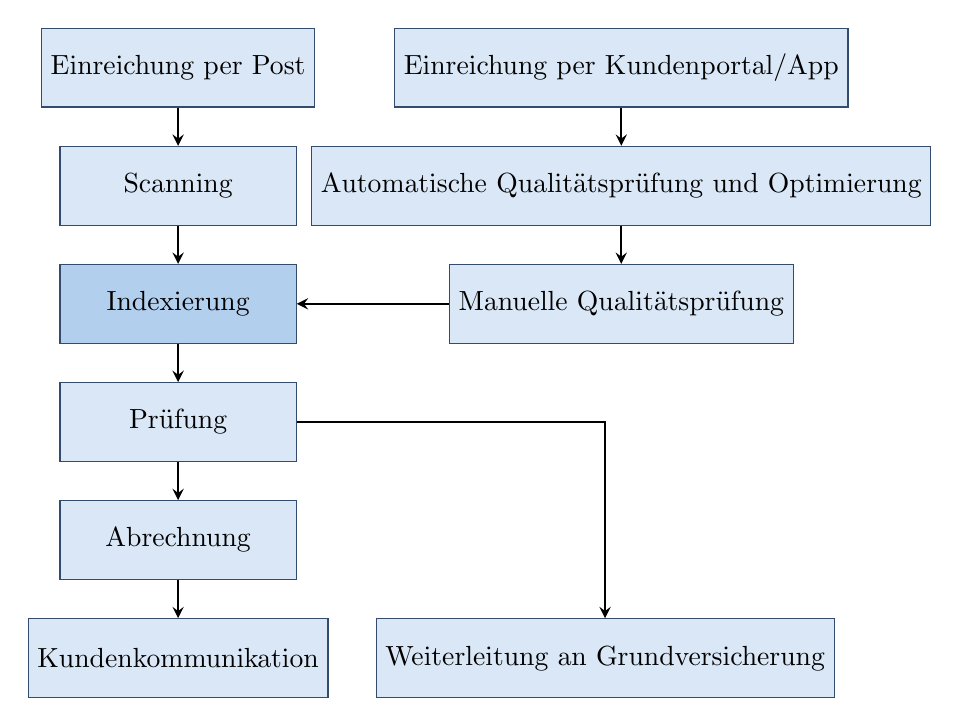
\begin{tikzpicture}[
      node distance=1.5cm and 15cm
    ]
        \node (startPost) [process] {Einreichung per Post};
        \node (scanning) [process, below of=startPost] {Scanning};
        \node (startPortal) [process, right=1cm of startPost] {Einreichung per Kundenportal/App};
        \node (rectification) [process, below of=startPortal] {Automatische Qualitätsprüfung und Optimierung};
        \node (qualityGate) [process, below of=rectification] {Manuelle Qualitätsprüfung};
        \node (indexing) [process2, below of=scanning] {Indexierung};
        \node (check) [process, below of=indexing] {Prüfung};
        \node (settlement) [process, below of=check] {Abrechnung};
        \node (communication) [process, below of=settlement] {Kundenkommunikation};
        \node (okp) [process, below of=check, right=1cm of settlement] {Weiterleitung an Grundversicherung};
        
        \draw [arrow] (startPost) -- (scanning);
        \draw [arrow] (scanning) -- (indexing);
        \draw [arrow] (startPortal) -- (rectification);
        \draw [arrow] (rectification) -- (qualityGate);
        \draw [arrow] (qualityGate) -- (indexing);
        \draw [arrow] (indexing) -- (check);
        \draw [arrow] (check) -- (settlement);
        \draw [arrow] (settlement) -- (communication);
        \draw [arrow] (check) -| (okp);
    \end{tikzpicture}
%\fi
\end{figure}

Die Entwicklung des Prototypen beschränkt sich auf den Prozessschritt der Indexierung. Die Einreichung sowie die Weiterverarbeitung der Rechnungen nach der Indexierung, sprich die Auswertung, ob und wie eine bestimmte Rechnungsposition versichert ist, ist nicht Teil des Prototypen.

% Für das Fallbeispiel wird ein Prototyp entwickelt, welcher die Indexierung der Rechnungen abdeckt. Für den Prototypen ist es als Ausgangslage wichtig, in welcher Form und Qualität die Rechnungen beim Krankenversicherer ankommen. Weiter ist es für die Zielsetzung wichtig, in welches Format die Rechnungen gebracht werden müssen, damit diese anschliessend weiterverarbeitet werden können. Diese beiden Aspekte sollen als Rahmenbedingungen für den Prototypen gelten.

\newpage
\section{Methodische Vorgehensweise}

\todo[inline]{
Hier wird die methodische Vorgehensweise zur Beantwortung der Forschungsfrage erläutert. Die Vorgehensweise bezieht sich auf die Art der empirischen Datenerhebung (qualitativ, quantitativ oder eine Mischform) wie auch auf die geplante Auswertung der erhobenen Daten. Methoden der Datenerhebung sind beispielsweise eine Umfrage oder Interviews, Methoden der Datenanalyse sind beispielsweise statistische Tests oder eine Inhaltsanalyse. Es wird beschrieben, wie bei der Datenerhebung und -analyse vorgegangen werden soll (wer soll wie befragt werden, wie werden die Daten analysiert) und welche kritischen Aspekte in der Erhebung und Analyse zu erkennen sind
}

\todo[inline, color=red]{Vorgehen klarer strukturiert und detaillierter beschreiben? (Verschiedene 
Zugänge zur Forschungsfrage? Wie genau entwickeln Sieden Prototyp? Wie
testen Sie Ihn? Wie erheben Sie welche Daten? Wie werten Sie die gewonnenen 
Daten aus? (Siehe Kommentare im pdf. Im Kapitel Vorgehen sehe ich den 
einzigen grösseren Optimierungsbedarf.)}

\todo[inline,color=green]{Modell mit Stufen (Texterkennung (OCR, Korrektur), Informationsextraktion (IE, Strukturierung) und "Selbstcheck" (prüfung ob ergebnis ok oder ob auslenken)

Kriterien/Erwartungen für einzelne Schritte definieren}

Kapitel 2 bietet einen literaturbasierten Zugang zur Forschungsfrage. Dabei wird erläutert, was eine erfolgreiche Automatisierung eines Geschäftsprozesses ausmacht. Weiter werden Versuche der Automatisierung, bei welchen künstliche Intelligenz zur Anwendung gekommen ist, diskutiert.

Im Kapitel 3 wird der aktuelle Forschungsstand im Gebiet der künstlichen Intelligenz präsentiert und Techniken aus diesem Bereich erläutert.
% Grobkzept: Forschungsstand

Der Hauptteil der Arbeit wird in Kapitel 4 abgehandelt. Es werden erst die Rahmenbedingungen für den Prototypen definiert und erläutert. Zu diesen Rahmenbedingungen gehören sowohl das Format und die Qualität der Rechnungen als auch die Erwartungen hinsichtlich Form und Qualität der Resultate. Damit der Prototyp bewertet werden kann, wird ein Set an Tests definiert. Folgend wird der Prototyp entwickelt. Dabei wird der Entwicklungsprozess dokumentiert. Der Abschluss bildet das Testen des Prototypen anhand der zuvor definierten Tests.

Schlussendlich wird anhand der Resultate aus der Literaturrecherche sowie dem Test des Prototypen die Forschungsfrage beantwortet. Weiter werden Empfehlungen abgeleitet.

Während die Forschungsfrage aufgrund existierender Literatur diskutiert wird, bildet der Prototyp, welcher zur Diskussion des Fallbeispiels entwickelt wird, eine zentrale Rolle bei der Beantwortung der Forschungsfrage.

\todo[inline, color=red]{Vorschlag: Vielleicht den Aspekt \enquote{learning by doing} erwähnen.}

\todo[inline, color=red]{Frage: Wer definiert die Erfolgskriterien? Machst Du das alleine? 

Hinweis: Bitte achte darauf, dass Du das Ganze objektiv machen kannst und dass diese Rahmenbedingungen und Erfolgskriterien valide sind. 

-> eine Möglichkeit: basierend auf Literatur (1:1)

- > andere Möglichkeit: adaptiert von Literatur, dann aber besprochen mit Experten}

\todo[inline, color=red]{Vorschlag: Evtl. wäre das Design Science Research Modell etwas für Dich? Siehe Anhang im Mail. Ich weiss aber nicht, ob ihr in der Schule etwas in diese Richtung schon angeschaut habt. :)}
 
\newpage
\section{Provisorisches Inhaltsverzeichnis} 

\todo[inline]{
Im provisorischen Inhaltsverzeichnis werden die thematischen Schwerpunkte der Thesis und welche wissenschaftlichen Theorien und Erklärungsansätze zur Beantwortung der Forschungsfrage herangezogen werden, definiert. Die Überschriften der Hauptkapitel der Thesis lassen die relevanten Teilaspekte des Themas und das methodische Vorgehen erkennen. Weitere Hinweise zum Aufbau der Thesis befinden sich in den Richtlinien für die Erstellung von Bachelor und Master Theses, Punkt 5.
}

{
    \renewcommand\labelitemi{--}
    \renewcommand{\labelenumi}{\arabic{enumi}}
    \renewcommand{\labelenumii}{\labelenumi.\arabic{enumii}}
    \renewcommand{\labelenumiii}{\labelenumii.\arabic{enumiii}}
    \begin{itemize}[topsep=0pt,itemsep=2pt,partopsep=4pt, parsep=4pt]
        \item Management Summary
        \item Ehrenwörtliche Erklärung
        \item Abkürzungsverzeichnis
    \end{itemize}
    \begin{enumerate}[topsep=0pt,itemsep=2pt,partopsep=4pt, parsep=4pt]
        \item Einleitung
        \item Grundlagen der künstlichen Intelligenz
        \begin{enumerate}[topsep=0pt,itemsep=2pt,partopsep=4pt, parsep=4pt]
            \item Lernstrategien
            \item Neuronale Netzwerke
            \item Natural Language Processing
        \end{enumerate}
        \item Künstliche Intelligenz in der Automatisierung \textit{(Literatur)}
        \item Entwicklung eines Prototypen zur Indexierung von Rechnungen \textit{(Praktisch)}
        \begin{enumerate}[topsep=0pt,itemsep=2pt,partopsep=4pt, parsep=4pt]
            \item Vorgehen
            \item Rahmenbedingungen
            \begin{enumerate}[topsep=0pt,itemsep=2pt,partopsep=4pt, parsep=4pt]
                \item Format und Qualität der Rechnungen
                \item Erwartetes Format und Qualität der Resultate
            \end{enumerate}
            \item Texterkennung durch LSTM Netzwerk
            \item Optimierung der Resultate der Texterkennung
            \item Informationsextraktion aus den OCR Resultaten
            \begin{enumerate}[topsep=0pt,itemsep=2pt,partopsep=4pt, parsep=4pt]
                \item Named Entity Recognition and Classification
                \item Text classificiation
                \item Extraktion aus standardisierten, semi-strukturierten Formaten
            \end{enumerate}
            \item Diskussion der Resultate
        \end{enumerate}
        \item Schlussfolgerungen
        \begin{enumerate}[topsep=0pt,itemsep=2pt,partopsep=4pt, parsep=4pt]
            \item Beantwortung der Forschungsfrage
            \item Handlungsempfehlungen
            \item Offene Fragen
            \item Ausblick
        \end{enumerate}
        \item Anhang
        \begin{enumerate}[topsep=0pt,itemsep=2pt,partopsep=4pt, parsep=4pt]
            \item Literaturverzeichnis
            \item Tabellen- und Abbildungsverzeichnis
            \item Sourcecode des Prototypen
        \end{enumerate}
    \end{enumerate}
}

\newpage
\section{Meilensteine}

\todo[inline]{
Hier werden die wichtigsten Arbeitsschritte vom Erstellen des Grobkonzeptes bis zur Abgabe der Bachelor Thesis als Meilensteine wiedergegeben und der Betreuungsperson 3 Besprechungstermine vorgeschlagen (siehe Punkt 2 der Spezifischen Regelungen für Bachelor Theses). Die Betreuungsperson bestätigt bei der Prüfung des Grobkonzeptes die Terminvorschläge oder schlägt andere Termine vor.
}
 
\begin{table}[h]
\centering
    \caption{Meilensteine}
    \renewcommand{\arraystretch}{1.25}
    \setlength{\tabcolsep}{15pt}
    \begin{tabular}{ | p{8cm} | l |}
    \hline
    \rowcolor{ccc} Was? & Wann? \\ \hline
    Erster Besprechungstermin auf Basis des ersten Entwurfs des Grobkonzeptes. & 13. November 2018 \\ \hline
    
    Literaturrecherche zum gewählten Thema fortführen und Grobkonzept finalisieren. & 28. November 2018 \\ \hline
    
    \rowcolor{orange} Eingabe des Namens der Betreuungsperson, des Grobkonzeptes, des Titels, und gegebenenfalls der Angaben zur externen Fachperson & 2. Dezember 2018 \\ \hline
    
    Prüfung der Betreuungsanfrage, des Titels und des Grobkonzeptes durch die Betreuungsperson & 17. Dezember 2018 \\ \hline
    
    Theorieteil verfassen und empirische Untersuchung vorbereiten & 15. Januar 2019 \\ \hline
    
    Zweiter Besprechungstermin nach Fertigstellung des Theorieteils und zur Gestaltung des Experimentes & Januar 2019 \\ \hline
    
    Erstellung und Auswertung des Prototypen & 15. März 2019 \\ \hline
    
    Dritter Besprechungstermin zur vorläufigen Beantwortung der Forschungsfrage & März 2019 \\ \hline
    
    Fertigstellung der gesamten Thesis & 1. April 2019 \\ \hline
    
    Korrektorat der Thesis durchführen und Feedback einarbeiten, Thesis drucken und binden lassen & 26. April 2019 \\ \hline
    
    \rowcolor{orange} Frist zur Abgabe und Hochladen der Bachelor Thesis & 3. Mai 2019 18:00 Uhr \\ \hline
    
    \end{tabular}
\end{table}


\newpage
\section{Erste Quellenverweise zum Thema}
\todo[inline]{
Hier werden bereits gelesene Quellen angeführt und auf weiterführende Literatur verwiesen, die noch ausgewertet wird.
}

{
    \nocite{Brynjolfsson2017Artificial}
    \nocite{BughinARTIFICIALFRONTIER}
    \nocite{ChuiFourAutomation}
    \nocite{Kolbjrnsrud2016HowManagement}
    \nocite{Tredinnick2017ArtificialRoles}
    \printbibliography[heading=none]
}

\newpage

\section{Anhang}

\makeBibliography{Anhang}{Literaturverzeichnis}

\newpage
\makeListOfTablesAndFigures{Tabellen- und Abbildungsverzeichnis}

\end{document}